\documentclass[10pt,twocolumn]{article}
\setlength\textwidth{6.875in}
\setlength\textheight{8.875in}
% set both margins to 2.5 pc
\setlength{\oddsidemargin}{-0.1875in}% 1 - (8.5 - 6.875)/2
\setlength{\evensidemargin}{-0.1875in}
\setlength{\marginparwidth}{0pc}
\setlength{\marginparsep}{0pc}%
\setlength{\topmargin}{0in} \setlength{\headheight}{0pt}
\setlength{\headsep}{0pt}
\setlength{\footskip}{37pt}%
\setlength{\columnsep}{0.3125in}
\setlength{\columnwidth}{3.28125in}% (6.875 - 0.3125)/2 = 3.28125in
\setlength{\parindent}{1pc}
\newcommand{\myMargin}{1.00in}
\usepackage[top=\myMargin, left=\myMargin, right=\myMargin, bottom=\myMargin, nohead]{geometry}
\usepackage{epsfig,graphicx}
\usepackage{palatino}
\usepackage{fancybox}

\newenvironment{commentary}
{ \vspace{-0.1in}
  \begin{quotation}
  \noindent
  \small \em
  \rule{\linewidth}{1pt}\\
}
{
  \end{quotation}
}

\title{Chisel Manual}
\author{Jonathan Bachrach, Krste Asanovi\'{c}, John Wawrzynek \\
EECS Department, UC Berkeley\\
{\tt  \{jrb|krste|johnw\}@eecs.berkeley.edu}
}
\date{\today}

\newenvironment{example}{\VerbatimEnvironment\begin{footnotesize}\begin{Verbatim}}{\end{Verbatim}\end{footnotesize}}
\newcommand{\kode}[1]{\begin{footnotesize}{\tt #1}\end{footnotesize}}

\def\code#1{{\tt #1}}

\def\note#1{\noindent{\bf [Note: #1]}}
%\def\note#1{}

\begin{document}
\maketitle{}

% TODO: default
% TODO: enum yields Bits
% TODO: why hardware construction languages

\section{Introduction}

This document is a manual for {\em Chisel} (Constructing
Hardware In a Scala Embedded Language).  Chisel is a hardware
construction language embedded in the high-level programming language
Scala.  Chisel is really only a set of special class
definitions, predefined objects, and usage conventions within Scala,
so when you write a Chisel program you are actually writing a Scala
program.  However, for the manual we don't presume that you
understand how to program in Scala.  We will point out necessary Scala
features through the Chisel examples we give, and significant hardware
designs can be completed using only the material contained herein.
But as you gain experience and want to make your code simpler or more
reusable, you will find it important to leverage the underlying power
of the Scala language. We recommend you consult one of the excellent
Scala books to become more expert in Scala programming.

\section{Nodes}

Chisel user code creates a graph of nodes which Chisel then translates
into Verilog or C++ code.  Nodes are defined as follows:

\begin{example}
class Node {
  var name: String = "";
  var isNamed = false; 
  def inputs: ArrayBuffer[Node];
  def consumers: ArrayBuffer[Node];
  def infer: Node => Int;
  def getWidth: Int;
  def getNode: Node;
  def toNode: Node;  
  def fromNode(Node): this.type; 
}
\end{example}

% TODO: toNode SHOULD BE toBits
% TODO: fromNode SHOULD BE fromBits

\noindent
where \verb+inputs+ and \verb+consumers+ are the incoming and
outgoing graph edges.

% explain getNode and types interspersed between nodes
% remove fromNode, toNode

\begin{figure}[h]
\centering
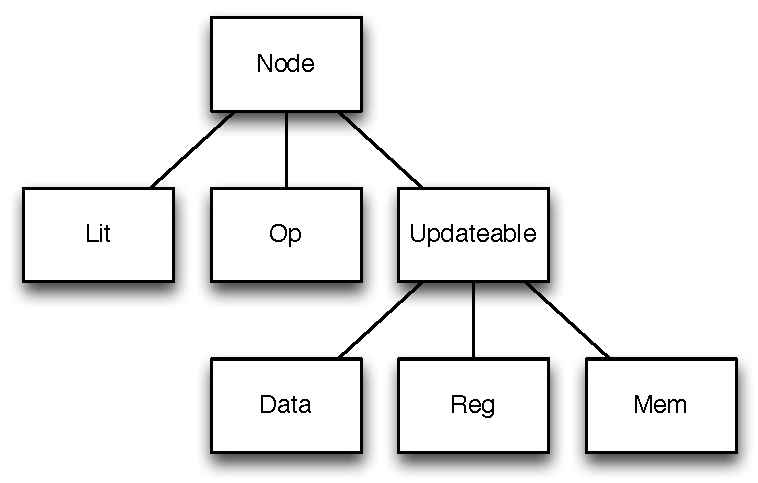
\includegraphics[width=3in]{figs/node-hierarchy.pdf}
\caption{Node hierarchy.}
\label{fig:node-hierarchy}
\end{figure}

\section{Lits}

Literal are represented as \verb+Lit+ nodes defined as follows:

\begin{example}
class Lit {
  val inputVal: BigInt;
}
\end{example}

\section{Ops}

Operations are represented as \verb+Op+ nodes defined as follows:

\begin{example}
class Op {
  val op: String;
}
\end{example}

\section{Types}

A Chisel graph contains port, op, and type nodes.  Type nodes are
interspersed between port and operator nodes and allow Chisel code to
check and respond to Chisel types.  Type nodes are erased before
emission to C++ and Verilog.  \verb+Type+ is the top most type node
and FIgure~\ref{fig:type-hierarchy}
shows the built in type hierarchy.

\begin{figure}[h]
\centering
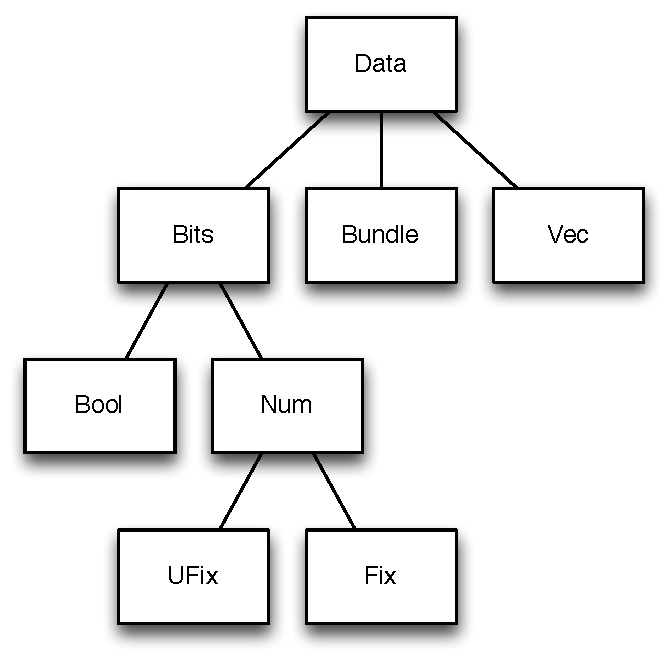
\includegraphics[height=2.5in]{figs/type-hierarchy.pdf}
\caption{Type hierarchy.}
\label{fig:type-hierarchy}
\end{figure}

\verb+Type+ itself is a node:

\begin{example}
abstract class Type extends Node {
  override def clone(): this.type =
    this.getClass.newInstance.asInstanceOf[this.type];
  def toFix: Fix;
  def toUFix: UFix;
  def toBits: Bits;
  def toBool: Bool;
  def flatten: Array[(String, IO)];
  def flip: this.type;
  def asOutput: this.type;
  def asInput: this.type;
  def :=[T <: Type](t: T);
  def <>(t: Type);
}
\end{example}

\noindent
with methods for converting between types and 
delegating port methods to its single input.   
We will discuss ports in Section~\ref{sec:ports}.
Finally, users can override this in their own type nodes (e.g., bundles) in
order to reflect construction parameters that are necessary for cloning.

% why not fromBits ?

\subsection{Bits}

In Chisel, a raw collection of
bits is represented by the \code{Bits} type defined as follows:

\begin{example}
object Bits {
  def apply(width: Int = -1): Bits;
  def apply(value: BigInt, width: Int = -1): Bits;
}

class Bits extends Type {
  def unary_-(): Bits;
  def unary_~(): Bits;
  def &  (b: Bits): Bits;
  def |  (b: Bits): Bits;
  def ^  (b: Bits): Bits;
  def andR(): Bool;
  def orR():  Bool;
  def && (b: Bool): Bool;
  def || (b: Bool): Bool;
  def ===(b: Bits): Bool;
  def != (b: Bits): Bool;
  def << (b: UFix): Bits;
  def >> (b: UFix): Bits;
  def ## (b: Bits): Bits;
}
\end{example}

\noindent
and with the simple bit operations.  
Bits with a value argument produces a \verb+Lit+ as shown in Figure~\ref{fig:bits-1}.
N.B., that \verb+##+ is binary
concatenation and \verb+===+ is bitwise comparison with \verb+==+.

Operations produce an
actual operator node and a type node combining the input type nodes.
See Figures~\ref{fig:bits-1}, \ref{fig:bits-and}, \ref{fig:bits-or-and} for
successively more complicated examples.

\begin{figure}[h]
\centering
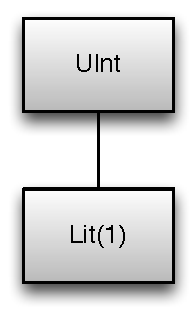
\includegraphics[height=1in]{figs/bits-1.pdf}
\caption{Chisel graph representing {\tt\footnotesize Bits(1)}.}
\label{fig:bits-1}
\end{figure}

\begin{figure}[h]
\centering
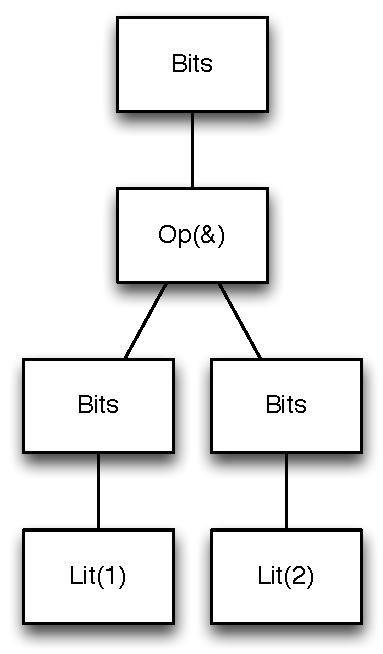
\includegraphics[height=1.5in]{figs/bits-and.pdf}
\caption{Chisel graph representing {\tt\footnotesize Bits(1)\&Bits(2)}.}
\label{fig:bits-and}
\end{figure}

\begin{figure}[h]
\centering
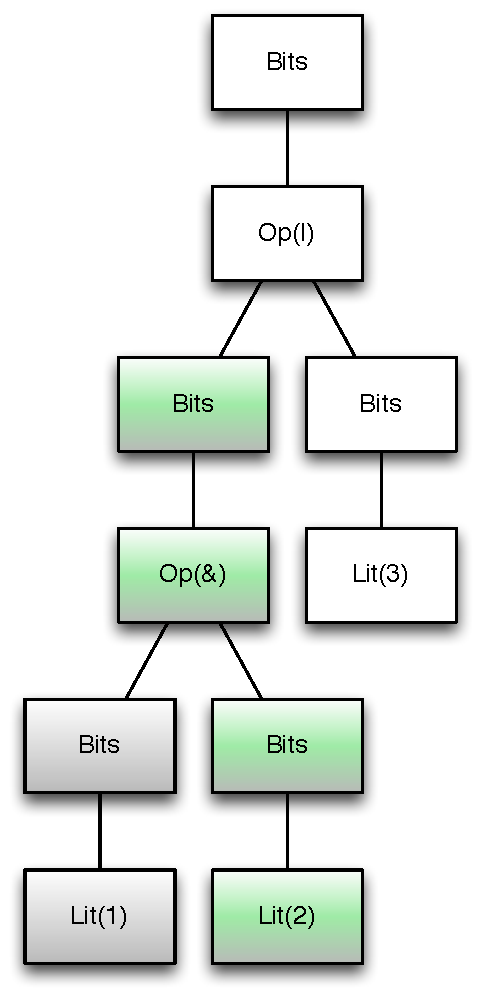
\includegraphics[height=2.5in]{figs/bits-or-and.pdf}
\caption{Chisel graph representing 
  {\tt\footnotesize (Bits(1)\&Bits(2))|Bits(3)} augmenting the graph
  shown in Figure~\ref{fig:bits-and}.}
\label{fig:bits-or-and}
\end{figure}

\noindent
The \verb+getNode+ operator will skip type nodes and return the first
non type node node.

\subsection{Bools}

Boolean values are represented as \code{Bool}:

\begin{example}
object Bool {
  def apply():Bool;
  def apply(value:Boolean): Bool;
}

class Bool extends Bits;
\end{example}

\subsection{Nums}

\verb+Num+ is a type node which defines arithmetic operations:

\begin{example}
class Num extends Bits {
  def +(b: Num): Num;
  def *(b: Num): Num;
  def -(b: Num): Num;
  def >(b: Num): Bool;
  def <(b: Num): Bool;
  def <=(b: Num): Bool;
  def >=(b: Num): Bool;
}
\end{example}

Signed and unsigned integers
are considered subsets of fixed-point numbers and are represented by
types \code{Fix} and \code{UFix} respectively:

\begin{example}
object Fix {
  def apply(width: Int = -1):Fix;
  def apply(value: BigInt, width: Int = -1): Fix;
}

class Fix extends Num; 

object UFix {
  def apply(width: Int = -1):UFix;
  def apply(value: BigInt, width: Int = -1): UFix;
}

class UFix extends Num; 
\end{example}

\noindent
Signed fixed-point
numbers, including integers, are represented using two's-complement
format.  

\subsection{Bundles and Vecs}

\code{Bundle} and \code{Vec} are classes that allow the user to expand
the set of Chisel datatypes with aggregates of other types.

Bundles group together several named fields of potentially different
types into a coherent unit, much like a \code{struct} in C 

\begin{example}
class Bundle extends Type {
  def elements: ArrayBuffer[(String, Type)];
}
\end{example}

\noindent
A user can get the names and Type corresponding to each element in a
Bundle with the \verb+elements+ method and recursively using the
\verb+flatten+ method. 
% TODO: perhaps flatten should be named allElements
Users can define their own by subclassing \verb+Bundle+ as follows:

\begin{example}
class MyFloat extends Bundle {
  val sign =  Bool();
  val exponent = Bits(width = 8);
  val significand =  Bits(width = 23);
}

val x = new MyFloat()
val xs = x.sign
\end{example}

Vecs create an indexable vector of elements: 

\begin{example}
object Vec {
  def apply[T <: Type](n: Int)(gen: => T): Vec[T];
}

class Vec[T <: Type](n: Int, val gen: () => T) 
    extends Type {
  def apply(idx: UFix): T
  def apply(idx: Int): T
}
\end{example}

\noindent
with \verb+n+ elements of type defined with the \verb+gen+ thunk.
Users can then either dynamically or statically accessed the elements.

% TODO: conditionally assigning to elements

\subsection{Bit Width Inference}

% TODO: perhaps IO should be renamed Port

Users are required to set bitwidths of ports and registers, but otherwise,
bit widths on wires are automatically inferred unless set manually by the user.
% TODO: how do you set the width explicitly?
The bit-width inference engine starts from the graph's input ports and 
calculates node output bit widths from their respective input bit widths according to the following set of rules:\\

{\footnotesize
\begin{tabular}{ll}
{\bf operation} & {\bf bit width} \\ 
\verb|z = x + y| & \verb|wz = max(wx, wy) + 1| \\
\verb+z = x - y+ & \verb|wz = max(wx, wy) + 1|\\
\verb+z = x & y+ & \verb+wz = max(wx, wy)+ \\
\verb+z = Mux(c, x, y)+ & \verb+wz = max(wx, wy)+ \\
\verb+z = w * y+ & \verb!wz = wx + wy! \\
\verb+z = x << n+ & \verb!wz = wx + maxNum(n)! \\
\verb+z = x >> n+ & \verb+wz = wx - minNum(n)+ \\
\verb+z = Cat(x, y)+ & \verb!wz = wx + wy! \\
\verb+z = Fill(n, x)+ & \verb+wz = wx * maxNum(n)+ \\
% \verb+z = x < y+ & \verb+<= > >= && || != ===+ & \verb+wz = 1+ \\
\end{tabular}
}
\\[1mm]
\noindent  
where for instance $wz$ is the bit width of wire $z$, and the \verb+&+
rule applies to all bitwise logical operations.

The bit-width inference process continues until no bit width changes.
Except for right shifts by known constant amounts, the bit-width
inference rules specify output bit widths that are never smaller than
the input bit widths, and thus, output bit widths either grow or stay
the same.  Furthermore, the width of a register must be specified by
the user either explicitly or from the bitwidth of the reset value.
From these two requirements, we can show that the bit-width inference
process will converge to a fixpoint.

\section{Wires}

We provide the declaration of a wire node that can be used immediately, 
but whose input will be set later:

\begin{example}
object Wire {
  def apply[T <: Type]()(gen: =>T): T;
  def apply[T <: Type](default: T): T;
}

class Wire extends Updateable;
\end{example}

%TODO: change proc to Updateable

\noindent
where \verb+Updateable+ collects accesses and code generates a mux
input for the wire:

\begin{example}
abstract Updateable extends Node {
  def reads: Queue[(Bool, UFix)];
  def writes: Queue[(Bool, UFix, Node)];
  def genMuxes(default: Node);
  def := (x: Node): this.type;
}
\end{example}

% TODO: is updateable 

\subsection{Conditional Updates}

When describing the operation of state
elements (and wires), it is often useful to instead specify when updates to the
registers (and wires) will occur and to specify these updates spread across
several separate statements.  Chisel provides conditional update rules
in the form of the \code{when} construct to support this style of
sequential logic description:

\begin{example}
object when {
  def apply(cond: Bool)(block: => Unit): when;
}
class when (prevCond: Bool) {
  def elsewhen (cond: Bool)(block: => Unit): when;
  def otherwise (block: => Unit): Unit;
}
\end{example}

Chisel provides some syntactic sugar for other common forms of
conditional updates:

\begin{example}
object unless {
  def apply(c: Bool)(block: => Unit) = 
    when (!c) { block )
}
\end{example}

\noindent and

\begin{example}
object otherwise {
  def apply(block: => Unit) = 
    when (Bool(true)) { block }
}
\end{example}

We introduce the \code{switch} statement for conditional updates
involving a series of comparisons against a common key:

\begin{example}
object switch {
  def apply(c: Bits)(block: => Unit): Unit;
}
object is {
  def apply(v: Bits)(block: => Unit);
}
\end{example}

\section{Ports}
\label{sec:ports}

Ports are wires used as interfaces to hardware components.  A port is
a directional wrapper for a primitive \code{Type} object.  

\begin{example}
trait PortDir;
object INPUT extends PortDir;
object OUTPUT extends PortDir;

class Port extends Wire {
  var dir: PortDir;
  override def flip;
}

object Input {
  def apply[T <: Type]()(gen: => T): T;
}
object Output {
  def apply[T <: Type]()(gen: => T): T;
}
\end{example}

\noindent
Aggregate ports can recursively be constructed using either a vec or
bundle with instances of \verb+Port+ as leaves.

\section{Regs}

\begin{example}
object Reg {
  def apply[T <: Type](t: T): T;
  def apply[T <: Type](t: T, resetVal: T): T;
  def apply[T <: Type](resetVal: T = null)(gen: =>T): T;
}
 
class Reg extends Updateable {
}
\end{example}

\section{Mems}

Chisel provides facilities for creating both read only and
read/write memories.  

\begin{example}
object Mem {
  def apply[T <: Type](depth: Int)(gen: => T): T;
}

class Mem[T <: Type](n: Int, gen: () => T) 
    extends Updateable {
  def apply(idx: UFix): T;
}

class MemRead[T <: Type]
      (val mem: Mem, val idx: UFix) 
    extends Node {
  def := (t: T): T;
}

class MemWrite[T <: Type]
      (val mem: Mem, val idx: UFix, val kind: T) 
    extends Node;
\end{example}

\section{Components}

In Chisel, {\em components} are very similar to {\em modules} in
Verilog, defining a hierarchical structure in the generated circuit.
The hierarchical component namespace is accessible in downstream tools
to aid in debugging and physical layout.  A user-defined component is
defined as a {\em class} which:
\begin{itemize}
\item inherits from \code{Component},
\item contains an interface Bundle stored in a field named \code{io}, and
\item wires together subcircuits in its constructor.
\end{itemize}

Users write their own components by subclassing Component which is
defined as follows:

\begin{example}
abstract class Component {
  val io: Bundle;
  def compileV: Unit;
  def compileC: Unit;
}
\end{example}

\begin{example}
val io = ...;
\end{example}

The \code{:=} assignment operator, used in the body of a
component definition, is a special operator in Chisel that wires the input of
left-hand side to the output of the right-hand side.  It is typically
used to connect an output port to its definition.

% is IO a good name?

The \verb+<>+ operator bulk connects interfaces of opposite gender.
Bulk connections connect leaf ports of the same name to each other.
After all connections are made and the circuit is being elaborated,
Chisel warns users if ports have other than exactly one connection to them.

\begin{example}
def <> (x: Node);
\end{example}

\subsection{Main}

The user calls chiselMain from their main object:

\begin{example}
object chiselMain {
  def apply[T <: Component]
    (args: Array[String], 
     gen: () => T, 
     scanner: T => TestIO = null, 
     printer: T => TestIO = null): T;
}
\end{example}

% TODO: TestIO

Command arguments are as follows:
\begin{tabular}{lll}
\verb+--target-dir+ & target pathname prefix \\
\verb+--gen-harness+ & generate harness file for C++ \\
\verb+--v+ & generate verilog \\
\verb+--vcd+ & enable vcd dumping \\
\verb+--debug+ & put all wires in class file \\
\end{tabular}

\section{C++ Emulator}

The C++ emulator is based on a fast multiword library using
C++ templates.  The \verb+dat_t+ represents multiple \verb+val_t+:

\begin{example}
typedef uint64_t val_t;
typedef int64_t sval_t; 
typedef uint32_t half_val_t;
\end{example}

\begin{example}
template <int w>
class dat_t {
 public:
  const static int n_words;
  inline int width ( void );
  inline int n_words_of ( void );
  inline bool to_bool ( void );
  inline val_t lo_word ( void );
  inline unsigned long to_ulong ( void );
  std::string to_str ();
  static dat_t<w> rand();
  dat_t<w> ();
template <int sw> 
  dat_t<w> (const dat_t<sw>& src);
  dat_t<w> (const dat_t<w>& src);
  dat_t<w> (val_t val);
template <int sw> 
  dat_t<w> mask(dat_t<sw> fill, int n);
template <int dw> 
  dat_t<dw> mask(int n);
template <int n> 
  dat_t<n> mask(void);
  dat_t<w> operator + ( dat_t<w> o );
  dat_t<w> operator - ( dat_t<w> o );
  dat_t<w> operator - ( );
  dat_t<w+w> operator * ( dat_t<w> o );
  dat_t<w+w> fix_times_fix( dat_t<w> o );
  dat_t<w+w> ufix_times_fix( dat_t<w> o );
  dat_t<w+w> fix_times_ufix( dat_t<w> o );
  dat_t<1> operator < ( dat_t<w> o );
  dat_t<1> operator > ( dat_t<w> o );
  dat_t<1> operator >= ( dat_t<w> o );
  dat_t<1> operator <= ( dat_t<w> o );
  dat_t<1> gt ( dat_t<w> o );
  dat_t<1> gte ( dat_t<w> o );
  dat_t<1> lt ( dat_t<w> o );
  dat_t<1> lte ( dat_t<w> o );
  dat_t<w> operator ^ ( dat_t<w> o );
  dat_t<w> operator & ( dat_t<w> o );
  dat_t<w> operator | ( dat_t<w> o );
  dat_t<w> operator ~ ( void );
  dat_t<1> operator ! ( void );
  dat_t<1> operator && ( dat_t<1> o );
  dat_t<1> operator || ( dat_t<1> o );
  dat_t<1> operator == ( dat_t<w> o );
  dat_t<1> operator == ( datz_t<w> o );
  dat_t<1> operator != ( dat_t<w> o );
  dat_t<w> operator << ( int amount );
  dat_t<w> operator << ( dat_t<w> o );
  dat_t<w> operator >> ( int amount );
  dat_t<w> operator >> ( dat_t<w> o );
  dat_t<w> rsha ( dat_t<w> o);
  dat_t<w>& operator = ( dat_t<w> o );
  dat_t<w> fill_bit(val_t bit);
  dat_t<w> fill_byte(val_t byte, int nb, int n);
template <int dw, int n> 
  dat_t<dw> fill( void );
template <int dw, int nw> 
  dat_t<dw> fill( dat_t<nw> n );
template <int dw> 
  dat_t<dw> extract();
template <int dw> 
  dat_t<dw> extract(val_t e, val_t s);
template <int dw, int iwe, int iws> 
  dat_t<dw> extract(dat_t<iwe> e, dat_t<iws> s);
template <int sw> 
  dat_t<w> inject
    (dat_t<sw> src, val_t e, val_t s);
template <int sw, int iwe, int iws> 
  dat_t<w> inject
    (dat_t<sw> src, dat_t<iwe> e, dat_t<iws> s);
template <int dw> 
  dat_t<dw> log2();
  dat_t<1> bit(val_t b);
  val_t msb();
template <int iw>
  dat_t<1> bit(dat_t<iw> b)
}
\end{example}

\begin{example}
template <int w, int sw> 
  dat_t<w> DAT(dat_t<sw> dat);
template <int w> 
  dat_t<w> LIT(val_t value);
template <int w> dat_t<w> 
  mux ( dat_t<1> t, dat_t<w> c, dat_t<w> a )
\end{example}

The Chisel compiler compiles top level components into a \verb+mod_t+
class that can be created and executed:

\begin{example}
class mod_t {
 public:
  std::vector< mod_t* > children;
  virtual void init (void) { };
  virtual void clock_lo (dat_t<1> reset) { };
  virtual void clock_hi (dat_t<1> reset) { };
  virtual void print (FILE* f) { };
  virtual bool scan (FILE* f) { return true; };
  virtual void dump (FILE* f, int t) { };
};
\end{example}

\begin{example}
environment variables
\end{example}

Either the Chisel compiler can create a harness or the user can write
a harness themselves.  The following is an example of a harness for a
CPU component:

\begin{example}
#include "cpu.h"

int main (int argc, char* argv) {
  cpu_t* cpu = new Cpu();  
  cpu->init();
  for (size_t t = 0; t < n; t++) {
    cpu->scan();
    cpu->clock_lo();
    cpu->clock_hi();
    cpu->print();
  }
}
\end{example}

\section{Verilog}

\begin{example}
running verilog backend
multiple modules
module name caching
\end{example}

\section{Standard Library}

\begin{example}
foldR
log2up
ispow2
Match
Reverse
PopCount
OHToUFix
UFixToOH
LFSR16
ShiftRegister
Mux1H
Arbiter
DecoupledIO
Queues
Pipes
\end{example}

% henry

% \section{Acknowlegements}
% 
% Many people have helped out in the design of Chisel, and we thank them
% for their patience, bravery, and belief in a better way.  Many
% Berkeley EECS students in the Isis group gave weekly feedback as the
% design evolved including but not limited to Yunsup Lee, Andrew
% Waterman, Scott Beamer, Chris Celio, etc.  Yunsup Lee gave us feedback
% in response to the first RISC-V implementation, called TrainWreck,
% translated from Verilog to Chisel.  Andrew Waterman and Yunsup Lee
% helped us get our Verilog backend up and running and Chisel TrainWreck
% running on an FPGA.  Brian Richards was the first actual Chisel user,
% first translating (with Huy Vo) John Hauser's FPU Verilog code to
% Chisel, and later implementing generic memory blocks.  Brian gave many
% invaluable comments on the design and brought a vast experience in
% hardware design and design tools.  Chris Batten shared his fast
% multiword C++ template library that inspired our fast emulation
% library.  Huy Vo became our undergraduate research assistant and was
% the first to actually assist in the Chisel implementation.  We
% appreciate all the EECS students who participated in the Chisel
% bootcamp and proposed and worked on hardware design projects all of
% which pushed the Chisel envelope.  We appreciate the work that James
% Martin and Alex Williams did in writing and translating network and
% memory controllers and non-blocking caches.  Finally, Chisel's
% functional programming and bit-width inference ideas were inspired by
% earlier work on a hardware description language called Gel~\cite{gel} designed in
% collaboration with Dany Qumsiyeh and Mark Tobenkin.
% 
% % \note{Who else?}
% 
% \begin{thebibliography}{50}
% \bibitem{gel} Bachrach, J., Qumsiyeh, D., Tobenkin, M. \textsl{Hardware Scripting in Gel}.
% in Field-Programmable Custom Computing Machines, 2008. FCCM '08. 16th.
% \end{thebibliography}
% 

\end{document}
